\documentclass[UTF8]{ctexart}
\usepackage[table]{xcolor}
\usepackage{algorithm}
\usepackage{algorithmic}
\usepackage{subfigure}
\usepackage{amsmath,bm}
\usepackage{fancybox}
\usepackage{listings}
\usepackage{xcolor}
\usepackage{diagbox}
\usepackage{amssymb}
\usepackage{amsmath}
\usepackage{amsthm}
\usepackage{empheq}
\usepackage{warpcol}
\usepackage{lscape}
\usepackage[framemethod=tikz]{mdframed}
\usepackage{mathtools}
\usepackage{fancyhdr} 
\usepackage{longtable,booktabs}                               
\usepackage{lastpage}                                           
\usepackage{layout} 


% 图表
\usepackage{array,multirow}
  \setlength\extrarowheight{2pt} % 行高增加
\usepackage{longtable}
\usepackage{graphicx}

\usepackage{listings}

\usepackage{xcolor}

	\definecolor{ocre}{RGB}{243,102,25}
	\definecolor{mygray}{RGB}{243,243,244}

%
%\lstset{
%columns=flexible,
%numbers=left,
%numberstyle=\footnotesize\color{darkgray}, 
%basicstyle=\small\ttfamily,
%stringstyle=\color{purple},
%keywordstyle=\color[RGB]{40,40,255}\bfseries,
%commentstyle=\it\color[RGB]{0,96,96},  
%stringstyle=\rmfamily\slshape\color[RGB]{128,0,0}, 
%showstringspaces=false,      
%% directivestyle=\color{blue},
%frame=shadowbox,
%%framerule=0pt,
%backgroundcolor=\color[RGB]{245,245,244},
%escapeinside=``, %逃逸字符(1左面的键),用于显示中文
%breaklines,
%extendedchars=false,
%%解决代码跨页时,章节标题,页眉等汉字不显示的问题
%xleftmargin=2em,xrightmargin=2em,
%aboveskip=1em,%设置边距
%tabsize=4, %设置tab空格数  
%showspaces=false %不显示空格 
%rulesepcolor=\color{red!20!green!20!blue!20}
%%rulesepcolor=\color{brown}
%}



% 行号
\usepackage{lineno}


% 引用
\usepackage[colorlinks=true,
            pdfborder=001,     
            citecolor=blue,
            linkcolor=red,
            anchorcolor=green,
            urlcolor=blue,
            bookmarksopen=true,bookmarksnumbered=true]{hyperref}
\usepackage{paralist}
\usepackage{minted}
\definecolor{bg}{rgb}{0.95,0.95,0.95}
\newtheorem{lemma}{引理}[section]
\title{高效稀疏编码算法}
\author{张晋}
\begin{document}
\maketitle

\section{稀疏编码}
\subsection{介绍}
稀疏编码是一种无监督学习方法,它通过寻找一组\textbf{过完备(overcomplete)}的基向量来更高效地表示样本数据。

具体来说,
若输入向量为$\vec{\xi}^ {(1)},\vec{\xi}^ {(2)},\ldots,\vec{\xi}^{(m)}$,
该算法要找到一组基向量$ \vec{b}_1,\ldots,\vec{b}_n\in\mathbb{R}^k \,(n>k)$,使得我们能将输入向量 $\vec{\xi}\in\mathbb{R}^k$ 表示为这些基向量的线性组合:
\begin{align}
\xi = \sum_{j=1}^n \vec{b}_j s_j
\end{align}

其中,$\vec{s}\in \mathbb{R}^n$是对应的稀疏系数向量。

虽然一组\textbf{完备}的基向量就可以将输入向量全部表示出来,并且很快很方便,例如主成分分析法(PCA),
但我们依旧选择\textbf{过完备基(overcomplete basis)},因为它能更有效地找出隐含在输入数据内部的结构与模式。

但在选择过完备基的同时,基向量的系数$\vec{s}$却不是唯一确定的了,为了使学到的特征更明显,我们需要给系数$\vec{s}$加上一个\textbf{稀疏性}的限制,那么我们可以定义代价函数为:
\begin{equation}\label{cost}
  \sum_{i=1}^{m} \Big[\frac{1}{2\sigma^2}\| \vec{\xi}^{(i)} - \sum_{j=1}^n \vec{b}_j s_j^{(i)}\|^2+ \beta \sum_{j=1}^{n}\phi(s_j^{(i)})\Big]
\end{equation}

其中$\beta$是常系数,$\phi(\cdot)$是稀疏代价函数,可以取以下任意一种:

\[\phi(s_j)=\begin{cases}
      \|s_j\|_1 & (\mbox{$L_1$罚函数 })  \\
      \sqrt{s_j^2+\epsilon} & \mbox{(epsilon$L_1$罚函数 )}  \\
      \log(1+s_j^2) & \mbox{(log罚函数)}.
    \end{cases}\]

本文中采用的是$L_1$罚函数,因为$L_1$正则化能产生稀疏系数,并且对不相关的特征具有鲁棒性。

此外,我们需要给$\vec{b}_j$加上一些约束条件,因为若$b$无约束,那么$b$就能在$s$线性减小的同时线性增大,并使得$\sum_{j=1}^n \vec{b}_j s_j^{(i)}$不变,最后$s\rightarrow0,b\rightarrow\infty$,这显然不是我们想要的结果。因此,我们需要限制$b$的大小:$\|\vec{b}_j\|^2 \leq c, \,\forall j = 1,...,n$.包含了限制条件的稀疏编码代价函数的完整形式如下:

\begin{equation}\label{opt1}
\begin{array}{rc}
\text{minimize}_{\{\vec{b}_j\},\{\vec{s}^{(i)}\}} & \sum_{i=1}^{m} \Big[\frac{1}{2\sigma^2}\| \vec{\xi}^{(i)} - \sum_{j=1}^n \vec{b}_j s_j^{(i)}\|^2+ \beta \sum_{j=1}^{n}\phi(s_j^{(i)})\Big]\\
\text{subject to}  &  \|\vec{b}_j\|^2 \leq c, \,\forall j = 1,...,n.
\end{array}
\end{equation}

可以将问题(\ref{opt1})表示成更简洁的矩阵形式,
记$X\in \mathbb{R}^{k\times m}$为输入向量$\vec{\xi}^ {(1)},\vec{\xi}^ {(2)},\ldots,\vec{\xi}^{(m)}$排成的矩阵;
记$B\in \mathbb{R}^{k\times n}$为基向量矩阵,由基向量$ \vec{b}_1,\ldots,\vec{b}_n$组成;
记$S\in \mathbb{R}^{n\times m}$为系数矩阵,由系数向量$\vec{s}^ {(1)},\vec{s} ^{(2)},\ldots,\vec{s}^{(m)}$组成。那么原优化问题(\ref{opt1})可以写成以下形式:

\begin{equation}\label{opt2}
\begin{array}{rc}
\text{minimize}_{B,S} & \frac{1}{2\sigma^2}\|X-BS\|_F^2
+ \beta \sum_{i,j}\phi(S_{i,j})\\
\text{subject to}  &  \sum_{i}B_{i,j}^2 \leq c, \,\forall j = 1,\ldots,n.
\end{array}
\end{equation}


\subsection{概率解释}
Olshausen 和 Field 在 1997年提出了这个基于超完备基的稀疏编码算法,
并从概率的角度解释了稀疏编码算法的\textbf{生成模型(generative model)}。

%他们一开始建模的对象是V1区简单细胞的感受野,
首先假定输入$\xi$是$n$个特征$\vec{b}_j$的线性组合,并加上高斯噪声$\nu$:
\begin{equation}
  \xi = \sum_{j=1}^n \vec{b}_j s_j+\nu(\xi)
\end{equation}

其中噪声$\nu$服从均值为0、协方差为$\sigma^2I$的高斯分布,那么有:
\begin{equation}
  P(X\mid B,S)=\dfrac{1}{2\pi\sigma}\text{exp}
\left(-\frac{1}{2\sigma^2}(X-BS)^{\top}(X-BS)\right)
\end{equation}

然后给定系数向量$s$一个先验分布$P(s)$,由于我们期望的$s$是稀疏的,所以先验分布$P(s)$通常取一个峰值很尖锐且接近0的分布。常见的有Laplace、Cauchy、Student-t分布。在此我们选择Laplace分布:
\begin{equation}
P(s_i)=\text{Laplace}(s_i;0,\frac{1}{\lambda})=\frac{\lambda}{2}
\text{e}^{-\lambda|s_i|}
\end{equation}

同时每个$s_i$之间都是独立的,因此:
\begin{equation}
  P(S)=\prod_{i=1}^{n}P(s_i)
\end{equation}

%标准生成模型BSC假定\textbf{重构误差(reconstruction error)}  $\vec{\xi}-\sum_j\vec{b}_js_j$ 服从均值为0、协方差为$\sigma^2I$的高斯分布.为了保证系数的稀疏性,系数$s_j$的先验分布定为$P(s_j)\propto \text{exp}(-\beta\phi(s_j))$\footnote{概率分布在零值附近是凸起的,而且峰值很高},

%给定由$m$个输入向量$\vec{\xi}^ {(1)},\vec{\xi}^ {(2)},\ldots,\vec{\xi}^{(m)}$组成的训练集,和对应的系数向量$\vec{s}^ {(1)},\vec{s} ^{(2)},\ldots,\vec{s}^{(m)}$。
对于基$B$可能的分布一无所知,所以根据\textbf{同等无知原则},先验地认为基服从均匀分布$P(B)=1/\theta$,那么基和系数的最大后验估计为:
\begin{align*}\label{bayes}
  [\hat{B},\hat{S}]_{MAP}(X)
& =\mathop{\arg\max}_{B,S}\frac{P( X\mid B,S)P(B)P(S)}{\iint_{\Theta}P( X\mid B',S')P(B')P(S')\textrm{d}B'\textrm{d}S'}\\
& =\mathop{\arg\max}_{B,S}P(X\mid B,S)P(S)\\
& =\mathop{\arg\max}_{B,S}\log P(X\mid B,S)+\log P(S)\\
& =\mathop{\arg\max}_{B,S}
-\frac{1}{2\sigma^2}(X-BS)^{\top}(X-BS)
-\lambda\sum_{j=1}^{n}\|s_j\|_1\\
& =\mathop{\arg\min}_{B,S}\frac{1}{2\sigma^2}\|X-BS\|_F^2+
\lambda\sum_{j=1}^{n}\|s_j\|_1
\end{align*}

不难看出,如果先验分布$P(s)$取柯西分布$P(s_j) = \beta/(1+s_j^2) $的话,那么得到的正则化项为$ \sum_{i=1}^{m}\sum_{j=1}^{n}\log(1+s_{i,j}^2)$,对应
稀疏代价函数$\phi(\cdot)$取log罚函数的情况。

同时,如果我们没有对$B,S$假定一个先验分布,而是直接求基与系数的极大似然估计$[\hat{B},\hat{S}]_{ML}(X)=\mathop{\arg\max}_{B,S} P(X\mid B,S )$的话,那么得到的就是没有罚函数项的重构误差代价函数。


\section{问题求解}
观察式(\ref{opt2}),可以看出当固定住$S$时,这是个关于$B$的凸优化问题,而固定住$B$时,这也是个关于$S$的凸优化问题,但是组合到一起时却是非凸的。因此考虑在固定住其中一个的情况下,对另一个进行迭代优化,并且采用交替着进行迭代优化的方法。

当固定住$S$时,问题(\ref{opt2})就成了一个带着二次约束的最小二乘问题,此时可以采用Lagrange对偶法将其化成无约束二次优化。

当固定住$B$时,问题(\ref{opt2})成了一个标准的LASSO(least absolute shrinkage and selection operator)问题,由于$L_1$正则化项不可微,所以许多直接基于梯度的优化方法都不可用,要解决这种问题,可以使用通用QP求解器(例如CVX)、内点法、修正最小角回归法(LARS)、嫁接法(grafting)等,但本文介绍一种新的方法——\textbf{特征符号搜索法(feature-sign search algorithm)}可以更高效地解决这个问题。

\subsection{系数的学习——特征符号搜索法}
\subsubsection{Motivation}
虽然L1项在0处不可微,但可以先对$x_i$的符号进行假设,
在此基础上消去绝对值,然后就可以求得子问题的最优解$x_{new}$,
并在线段$x_c$到$x_{new}$之间进行线搜索,
为了减小计算量和保证稀疏性,只需要搜索在线段与坐标平面的交点即可,然后在里面找出原问题的最优点,
由于子问题也是原问题的众多种情况之一,因此在子问题中
通往最优解的这条线段上,也能找到点在原问题中是下降的。
得到新解后,根据已知信息对符号进行合理的假设,以保障下一次的迭代也会下降。最后由于$x$符号的状态有限,加上每一次都是严格下降的,所以最终一定能收敛到最优解。

\subsubsection{子问题}
对于原问题:
\begin{equation}\label{opt3}
\begin{array}{rc}
\text{minimize}_{x} &
f(x)\equiv \|y-Ax\|^2+\gamma\|x\|_1
\end{array}
\end{equation}

特征符号搜索法通过维持一个非零系数的积极集并记录其系数的符号来
使问题得到简化:用\emph{active set}记录非零系数的标号,用$\theta_i\in\{-1,0,1\}$记录$x_i$的符号,
那么$\gamma\|x\|_1$就可以表示为$\gamma\theta^{\top}x$,
用$\hat{x}$表示$x$中非零的子向量,$\hat{\theta}$是对应的符号向量,那么$\gamma\theta^{\top}x$可以进一步简化为$\gamma\hat{\theta}^{\top}\hat{x}$,再用$\hat{A}$表示$A$中对应的子矩阵,原优化问题就转化成了以下优化问题:

\begin{equation}\label{opt4}
\begin{array}{rc}
\text{minimize}_{\hat{x}} &
f(x)\equiv \|y-\hat{A}\hat{x}\|^2+\gamma\hat{\theta}^{\top}\hat{x}
\end{array}
\end{equation}

\[\nabla f=-2\hat{A}^{\top}(y-\hat{A}\hat{x})+\gamma\hat{\theta}\]

令$\nabla f=0$解得\footnote{前提是$\hat{A}$列满秩。若$\hat{A}^{\top}\hat{A}$是奇异的,首先检查是否$\hat{A}^{\top}y-\gamma\hat{\theta}/2\in \mathcal{R}(\hat{A}^{\top}\hat{A})$,若成立,则说明有解,只是解不唯一,此时可以用伪逆来代替;若不成立,说明无解,此时朝任一满足条件$z\in\mathcal{N}(\hat{A}^{\top}\hat{A})$的方向$z$移动$\hat{x}$,直到其与坐标平面相交,然后更新$\hat{x}$。这两种情况对于目标函数都是严格下降的,因此算法的收敛性不变。}


\[\hat{x}=(\hat{A}^{\top}\hat{A})^{-1}
(\hat{A}^{\top}y-\gamma\hat{\theta}/2)\]



\subsubsection{具体算法}
\begin{algorithm}[h]
\caption{特征符号搜索法}
\label{FSS_algorithm}
\begin{algorithmic}[1]
\STATE 初始化$x:=\vec{0},\,\theta:=\vec{0}$,积极集$\emph{active set}:=\{\}.$
\STATE 从值为0的$x_i\in x$中,选出$i=\arg \max_i \Big|\frac{\partial \|y-Ax\|^2}{\partial x_i}\Big|$.\\
 如果$x_i$的变动能使目标值减小,那就把$i$添加到积极集中去:\\
 $\quad$若$\frac{\partial \|y-Ax\|^2}{\partial x_i}>\gamma$
,令$\theta_i:=-1,\emph{active set}:=\{i\}\bigcup\emph{active set}.$\\
$\quad$若$ \frac{\partial \|y-Ax\|^2}{\partial x_i}<-\gamma$
,令$\theta_i:=1,\emph{active set}:=\{i\}\bigcup\emph{active set}.$
\STATE 特征符号步\\
$\quad$求解子问题(\ref{opt4}),得到解
$\hat{x}_{new}=(\hat{A}^{\top}\hat{A})^{-1}
(\hat{A}^{\top}y-\frac{1}{2}\gamma\hat{\theta})$\\
$\quad$在$\hat{x}$到$\hat{x}_{new}$的闭线段上进行离散的线搜索:\\
$\qquad$找到$\hat{x}_{new}$和所有改变符号处的点,即zero-crossing点:\\$\qquad \qquad \hat{x}-\dfrac{\hat{x} _j}{(\hat{x}_{new})_j-\hat{x}_j}(\hat{x}_{new}-\hat{x}),\quad j\in \emph{active set}$\\
$\qquad$计算在这些点处的目标函数值,并取最小值点作为更新\\
$\quad$从\emph{active set}中删去新解$\hat{x}$中值为0的指标,并更新$\theta=\text{sign}(x)$
\STATE 检查最优性条件 \\
$\quad(a)$对非零系数:$\frac{\partial \|y-Ax\|^2}{\partial x_j}+\gamma\,\text{sign}(x_j)=0,\quad \forall x_j\neq0$\\
$\qquad\,\,$如果不符合条件(a),转到第3步;否则检查条件(b)\\
$\quad(b)$对零系数:$\Big|\frac{\partial \|y-Ax\|^2}{\partial x_i}\Big|\leq \gamma,\quad \forall x_j=0$\\
$\qquad\,$如果不符合条件(b),转到第2步;否则返回$x$作为最优解。
\end{algorithmic}
\end{algorithm}

\subsubsection{收敛性证明}
\begin{lemma}\label{lemma1}
  将在第3步开始时的解记为$x_c$,若其符号与$\theta$保持一致且不是问题(\ref{opt4})的最优解,算法保证第3步更新后的解对于目标值来说是严格下降的。
\end{lemma}
\begin{proof}
  记$\hat{x}_c$是$x_c$的非零子向量,考虑一个关于$\hat{x}$的光滑二次函数$\tilde{f}(\hat{x})=\|y-\hat{A}\hat{x}\|^2+\gamma\hat{\theta}^{\top}\hat{x}$.由于$\hat{x}_c$不是$\tilde{f}$的最优点,故有$\tilde{f}(\hat{x}_{new})<\tilde{f}(\hat{x}_c)$.现在有两种情况:
  \begin{compactenum}
    \item 若$\hat{x}_{new}$跟原积极集及符号向量一致,显然$\hat{x}_{new}$更优, 更新$\hat{x}_c=\hat{x}_{new}$
    \item $\hat{x}_{new}$跟原积极集及符号向量不一致,这说明$\hat{x}_c$到$\hat{x}_{new}$的闭线段必然穿过了坐标平面,取$\hat{x}_d$为该线段与坐标平面第一个相交的点(也就是说$\hat{x}_d$中只有一个维度的值变成了0,其它维度的符号与原符号向量保持一致),显然$\hat{x}_c\neq\hat{x}_d$,由$\tilde{f}$的凸性可知$\tilde{f}(\hat{x}_d)<\tilde{f}(\hat{x}_c)$\footnote{$\hat{x}_{new}$是凸函数$\tilde{f}$的极小点,而$\tilde{f}(\hat{x} _d)$又在$\hat{x}_c$到$\hat{x}_{new}$的线段上,因此$\hat{x}_d$处的目标函数值严格比$\hat{x}_c$处的小},由于$\hat{x}_d$没有变号,故有$f(\hat{x}_d)=\tilde{f}(\hat{x}_d)<\tilde{f}(\hat{x}_c)=f(\hat{x}_c)$
  \end{compactenum}
\end{proof}

\begin{lemma}\label{lemma2}
  将在第2步开始时的解记为$x_c$,若其是问题(\ref{opt4})的最优解并且不是问题(\ref{opt3})的最优解,算法保证第3步更新后的解对于目标值来说是严格下降的
\end{lemma}
\begin{proof}
  由于$x_c$是问题(\ref{opt4})的最优解,所以其必然满足最优性条件(a),但其又不是问题(\ref{opt3})的最优解,所以必然不满足最优性条件(b);因此必然存在一个或多个$i$使得$\Big|\frac{\partial \|y-Ax\|^2}{\partial x_i}\Big|> \gamma$,不妨记第2步中添加到积极集\emph{active set}中的指标为$i$。

在第3步中,记$\tilde{f}(\hat{x})=\|y-\hat{A}\hat{x}\| ^2+\gamma\hat{\theta}^{\top}\hat{x}$,那么有:

\begin{compactenum}
\item 将$\tilde{f}$在$\hat{x}_c$处展开,其一阶项只有$x_i$(由最优性条件(a),其他$x_j$的一阶偏导都为0),又由第2步可知:若$\nabla \tilde{f}>0$,则$\theta_i=-1$,若$\nabla \tilde{f}<0$,则$\theta_i=1$,记$\vec{a}=(0,\cdots,0,\theta_i,0,\cdots,0)^{\top}$,则有$-\nabla \tilde{f}//\vec{a}$,即$\tilde{f}$的下降方向$\vec{p}$与$\vec{a}$夹锐角,那么任一沿$\vec{p}$方向上的点$\hat{x}=\hat{x}_c+\alpha\vec{p}$中$x_i$项的系数为$\alpha p_i$,因为$\alpha p_i\theta_i>0$,故沿$\tilde{f}$下降方向更新会使得$\hat{x}_i$的符号与$\theta$保持一致。
\item 由于$\hat{x}_c$不是$\tilde{f}$的最优点,由$\tilde{f}$的凸性,在$\hat{x}_c$点处沿着$\hat{x}_{new}-\hat{x}$方向必然使$\tilde{f}$严格下降。
\end{compactenum}

综上:在线段$\hat{x}_c$到$\hat{x}_{new}$上的点的符号必然与$\theta$保持一致,由符号一致可以得出$\tilde{f}=f$,那么使$\tilde{f}$严格下降的点也必然会使$f$严格下降。
\end{proof}

\begin{lemma}\label{lemma3}
  本算法能保证在有限步之内收敛到问题(\ref{opt3})的全局极小点
\end{lemma}

\begin{proof}
  对第2步开始时的解$x_c$,无论$x_c$是由第1步初始化得来还是由第4步(b)转来,$x_c$都是满足最优性条件(a)的,那么由引理\ref{lemma2}可知第3步后得到的解必然严格下降。

对第3步开始时的解$x_c$,若它是由第2步得来,那么上面论证过在第3步结束后的解其必然能严格下降;若它是由第4步(a)转来,那么它的符号必然与$\theta$保持一致,由引理\ref{lemma2}可知第3步结束后得到的解必然严格下降

由于积极集\emph{active set}和符号向量$\theta$的组合的状态数目是有限的,再加上每一次迭代都使得目标值严格下降,因此迭代不会存在循环,必然在有限步之内得到最优解停止迭代。
\end{proof}

此外,$x$的初始值不一定非得为$\vec{0}$,任意初始值都可以,但是在根据$x$初始化完$\theta$和\emph{active set}后,需要跳过第2步,直接从第3步开始。

\subsection{基的学习——Lagrange对偶法}
当固定住$S$时,问题(\ref{opt2})可以简化为以下问题:
\begin{equation}\label{opt5}
\begin{array}{rc}
\text{minimize}_{B} &
\|X-BS\|_F^2\\
\text{subject to}  &  \sum_{i=1}^{k}B_{i,j}^2 \leq c, \,\forall j = 1,...,n.
\end{array}
\end{equation}

记$\Lambda=\text{diag}(\vec{\lambda})$,可以使用Lagrange对偶法来解决该优化问题:\footnote{
在下面的运算中要用到\textbf{迹(trace)}的以下性质:
\begin{compactenum}
\item $\textrm{d}f=\sum_{i,j}\dfrac{\partial f}{\partial X_{ij}}\text{d}X_{ij}=\text{tr}\left(\dfrac{\partial f}{\partial X}^T\text{d}X\right)$
\item $\textrm{d}(\text{tr}(X)) = \text{tr}(\textrm{d}X)$
\item $\mathrm{tr}(A^T) = \mathrm{tr}(A)$
\item 对尺寸相同的矩阵$A,B$有:$\text{tr}(A^{\top}B)=\sum_{i,j}A_{ij}B_{ij}=\text{tr}(BA^ {\top})$
\item 对尺寸相同的方阵$A,B,C$有:
$\text{tr}(ABC)=\text{tr}(ACB)=\text{tr}(BAC)$
\end{compactenum}}



\begin{equation}\label{opt6}
\begin{array}{rl}
  \mathcal{L}(B,\vec{\lambda})&=\text{tr}\Big((X-BS)^{\top}(X-BS)\Big)
+\sum_{j=1}^{n}\lambda_j(\sum_{i=1}^{k}B_{i,j}^2-c)\\
   &= \text{tr}\Big((X-BS)^{\top}(X-BS)\Big)
+\text{tr}(\Lambda B^{\top}B-c\Lambda)
\end{array}
\end{equation}

\begin{equation}\label{opt7}
\begin{array}{rl}
  \textrm{d}\mathcal{L}&=\text{tr}\Big((-dBS)^{\top}(X-BS)
+(X-BS)^{\top}(-dBS)+\Lambda dB^{\top}B+\Lambda B^{\top}dB\Big)\\
 &=\text{tr}\Big(-2S(X-BS)^{\top}dB+2\Lambda B^{\top}dB\Big)\\
&=\text{tr}\Big(\big(-2(X-BS)S^{\top}+2 B\Lambda ^{\top}\big)^{\top}dB\Big)
\end{array}
\end{equation}

\begin{align}
  \dfrac{\partial \mathcal{L}}{\partial B}&=-2(X-BS)S^{\top}+2 B\Lambda ^{\top}=0\\ \Rightarrow \quad B&=XS^{\top}(\Lambda+SS^{\top})^{-1}
\end{align}
将$B=XS^{\top}(\Lambda+SS^{\top})^{-1}$代入式(\ref{opt6})中得:
\begin{align*}
  \mathcal{L} & =\text{tr}\Big(X^{\top}X-X^{\top}BS-S^{\top}B^{\top}X+S^{\top}B^{\top}BS
+\Lambda B^{\top}B-c\Lambda\Big) \\
   & =\text{tr}\Big(X^{\top}X-2BSX^{\top}+B^{\top}BSS^{\top}
+ B^{\top}B\Lambda-c\Lambda\Big) \\
   &= \text{tr}\Big(X^{\top}X-2BSX^{\top}+B^{\top}XS^{\top}-c\Lambda\Big)\\
&= \text{tr}\Big(X^{\top}X-BSX^{\top}-c\Lambda\Big)\\
&=\text{tr}\Big(X^{\top}X-XS^{\top}(SS^{\top}+\Lambda)^{-1}
(XS^{\top})^{\top}-c\Lambda\Big)
\end{align*}

\begin{equation}\label{Dlambda}
  \mathcal{D}(\vec{\lambda})=\min\limits_B   \mathcal{L}(B,\vec{\lambda})=
\text{tr}\Big(X^{\top}X-XS^{\top}(SS^{\top}+\Lambda)^{-1}
(XS^{\top})^{\top}-c\Lambda\Big)
\end{equation}

\begin{align}
  d\mathcal{D}(\vec{\lambda})&=\text{tr}\Big(\big(XS^{\top}(SS^{\top}+\Lambda)^{-2}
(XS^{\top})^{\top}-c\big)d\Lambda\Big)\\
\Rightarrow\quad \dfrac{\partial\mathcal{D}(\vec{\lambda})}{\partial \Lambda}&=\|XS^{\top}(SS^{\top}+\Lambda)^{-1}\|_F^2-c
\end{align}

\begin{align}\label{grad}
   \dfrac{\partial\mathcal{D}(\vec{\lambda})}{\partial \lambda_i}&=\Big(\|XS^{\top}(SS^{\top}+\Lambda)^{-1}\|_F ^2\Big)_{i,i}-c\nonumber\\
&=\|XS^{\top}(SS^{\top}+\Lambda)^{-1}e_i\|_2^2-c
\end{align}

\begin{align*}
d\Big(\dfrac{\partial\mathcal{D}(\vec{\lambda})}{\partial \lambda_i}\Big)&=d\Big(e_i^{\top}(SS^{\top}+\Lambda)^{-1}(XS^{\top})^{\top}(XS^{\top})(SS^{\top}+\Lambda)^{-1}e_i\Big)\\
&=-\text{tr}\Big(e_i^{\top}(SS^{\top}+\Lambda)^{-2}d\Lambda(XS^{\top})^{\top}(XS^{\top})(SS^{\top}+\Lambda)^{-1}e_i+\\
&\qquad e_i^{\top}(SS^{\top}+\Lambda)^{-1}(XS^{\top})^{\top}(XS^{\top})(SS^{\top}+\Lambda)^{-2}d\Lambda e_i\Big)\\
&=-2\text{tr}\Big((XS^{\top})^{\top}(XS^{\top})(SS^{\top}+\Lambda)^{-1}e_ie_i^{\top}(SS^{\top}+\Lambda)^{-2}d\Lambda \Big)
\end{align*}

\begin{equation}
   \dfrac{\partial \Lambda}{\partial \lambda_j}=e_je_j^{\top}
\end{equation}

\begin{align}\label{hess}
  \dfrac{\partial^2\mathcal{D}(\vec{\lambda})}{\partial \lambda_i\lambda_j} & =-2\text{tr}\Big((XS^{\top})^{\top}(XS^{\top})(SS^{\top}+\Lambda)^{-1}e_ie_i^{\top}(SS^{\top}+\Lambda)^{-2}e_je_j^{\top} \Big) \nonumber\\
   & =-2\text{tr}\Big((SS^{\top}+\Lambda)^{-1}(XS^{\top})^{\top}(XS^{\top})(SS^{\top}+\Lambda)^{-1}e_ie_i^{\top}(SS^{\top}+\Lambda)^{-1}e_je_j^{\top} \Big) \nonumber\\
   & =-2\text{tr}\Big(e_j^{\top}(SS^{\top}+\Lambda)^{-1}(XS^{\top})^{\top}(XS^{\top})(SS^{\top}+\Lambda)^{-1}e_ie_i^{\top}(SS^{\top}+\Lambda)^{-1}e_j \Big)\nonumber\\
&=-2e_j^{\top}(SS^{\top}+\Lambda)^{-1}(XS^{\top})^{\top}(XS^{\top})(SS^{\top}+\Lambda)^{-1}e_ie_i^{\top}(SS^{\top}+\Lambda)^{-1}e_j\nonumber\\
&=-2\Big(e_i^{\top}(SS^{\top}+\Lambda)^{-1}(XS^{\top})^{\top}(XS^{\top})(SS^{\top}+\Lambda)^{-1}e_j\Big)\Big(e_i^{\top}(SS^{\top}+\Lambda)^{-1}e_j\Big)\nonumber\\
&=-2\big((SS^{\top}+\Lambda)^{-1}(XS^{\top})^{\top}(XS^{\top})(SS^{\top}+\Lambda)^{-1}\big)_{i,j}\big((SS^{\top}+\Lambda)^{-1}\big)_{i,j}
\end{align}

Lagrange对偶法需要极大化式(\ref{Dlambda})中$\mathcal{D}(\vec{\lambda})$,
而在上面的式(\ref{grad})和式(\ref{hess})中我们分别计算出了式(\ref{Dlambda})中$\mathcal{D}(\vec{\lambda})$的梯度与Hessian阵,因此可以采用一些梯度方法如牛顿法或共轭梯度法来进行优化。

当确定了$\mathcal{D}(\vec{\lambda})$的极大值点$\lambda_1,\ldots,\lambda_n$后,可以求得最优基$B$为:
\begin{equation}\label{B}
  B=XS^{\top}(\Lambda+SS^{\top})^{-1}
\end{equation}

由于这一类优化问题的稀疏性:$n>k$,因此转化为对偶问题后需要优化的变量(Lagrange乘子)的个数大大减少。

此外,由于基的学习不涉及稀疏惩罚项,因此稀疏函数$\phi(\cdot)$的选择不影响本问题的求解。

\section{实验}
\subsection*{实验简述}
本实验使用稀疏编码来对图像进行编码的学习,
这需要解决两个一般性的凸优化问题:
\begin{itemize}
\item \textbf{L1正则化最小二乘问题}——使用特征符号搜索法解决
\item \textbf{L2约束最小二乘问题}——使用Lagrange对偶转化为无约束QP后使用共轭梯度法求解。
\end{itemize}

实验代码来源于Honglak Lee的\href{http://ai.stanford.edu/~hllee/softwares/nips06-sparsecoding.htm} {高效稀疏编码算法论文主页},实验数据来源于Olshausen为他1996年的那篇开创性论文编写的\href{http://www.rctn.org/bruno/sparsenet/}{稀疏编码仿真程序主页}。


\subsection*{文件说明}
\begin{itemize}
\item \texttt{demo\_fast\_sc.m} 整个实验的主程序框架
\item \texttt{IMAGES.mat}实验数据集
\item \texttt{getdata\_imagearray.m}将图片转换为输入参数
\item \texttt{sparse\_coding.m}进行稀疏编码的学习
\item \texttt{l1ls\_featuresign.m}使用特征符号搜索法学习稀疏系数$S$
\item \verb"cgf_fitS_sc2.m"使用共轭梯度法学习稀疏系数$S$(不可用)
\item \verb"l2ls_learn_basis_dual.m"使用Lagrange对偶学习基$B$
\item \verb"getObjective2.m"计算目标函数值(重构误差+稀疏惩罚)
\item \verb"display_figures.m"输出图像
\item \verb"save_figures.m"保存实验结果
\end{itemize}

\subsection*{代码改动说明}
由于代码是作者2007年编写的,而着期间MATLAB版本改动较大,因此需要作出以下调整:
\begin{enumerate}
  \item 将\texttt{demo\_fast\_sc.m}中第6行的
\begin{minted}[bgcolor=bg]{matlab}
opt_choice = 1;
\end{minted}
改为
\begin{minted}[bgcolor=bg]{matlab}
opt_choice = 2;
\end{minted}
  \item 将\texttt{demo\_fast\_sc.m}中第10行的
\begin{minted}[bgcolor=bg]{matlab}
load ../data/IMAGES.mat
\end{minted}
改为
\begin{minted}[bgcolor=bg]{matlab}
load ./data/IMAGES.mat
\end{minted}
  \item 将\texttt{sparse\_coding.m}中第34行的
\begin{minted}[bgcolor=bg]{matlab}
options = optimset('GradObj','on', 'Hessian','on');
\end{minted}
改为
\begin{minted}[bgcolor=bg,breaklines,
               breakanywhere,]{matlab}
options = optimset('Algorithm','trust-region-reflective' ,'GradObj','on', 'Hessian','on');
\end{minted}



  \item 此外,文件夹\verb"fast_sc\code\sc2"中的\texttt{cgf\_sc2.dll}是由32位MATLAB编译的,因此在64位的MATLAB中无法运行。而这个dll将在\verb"cgf_fitS_sc2.m"中被调用来进行共轭梯度法的计算,因此在64位的MATLAB中调用\verb"cgf_fitS_sc2.m"时会报错。
\end{enumerate}

\subsection*{实验步骤}
\begin{enumerate}
\item 使用\verb"cd"命令将路径更改到文件当前目录处
\item 在MATLAB命令行窗口输入\mintinline{matlab}{demo_fast_sc.m(2)},这意味着你使用特征搜索法调用程序\texttt{l1ls\_featuresign.m}来进行系数$S$的学习。

如果输入
\mintinline{matlab}{demo_fast_sc.m(1)}的话,意味着使用共轭梯度法调用程序\verb"cgf_fitS_sc2.m"来进行系数$S$的学习(会报错)。

也可以直接运行\verb"demo_fast_sc.m"程序,它将默认选择特征搜索法。

\item 程序内部每迭代一次会在命令行窗口输出当前信息,并弹出图片展示迭代情况,当100次迭代结束或达到终止条件后,程序将自动停止,并保存信息在文件夹\verb"fast_sc\results"中。
\end{enumerate}

\subsection*{实验结果展示}
在文件夹\verb"fast_sc\results"中可以找到以\verb".mat"为后缀的文件,将其拖入MATLAB命令行窗口,就能自动载入参数信息。然后在命令行输入:
\begin{minted}[bgcolor=bg,breaklines,
               breakanywhere,]{matlab}
display_figures(pars, stat, B, B, t)
\end{minted}
就能将迭代情况用图像展示出来:

\begin{figure}[H]
\centering
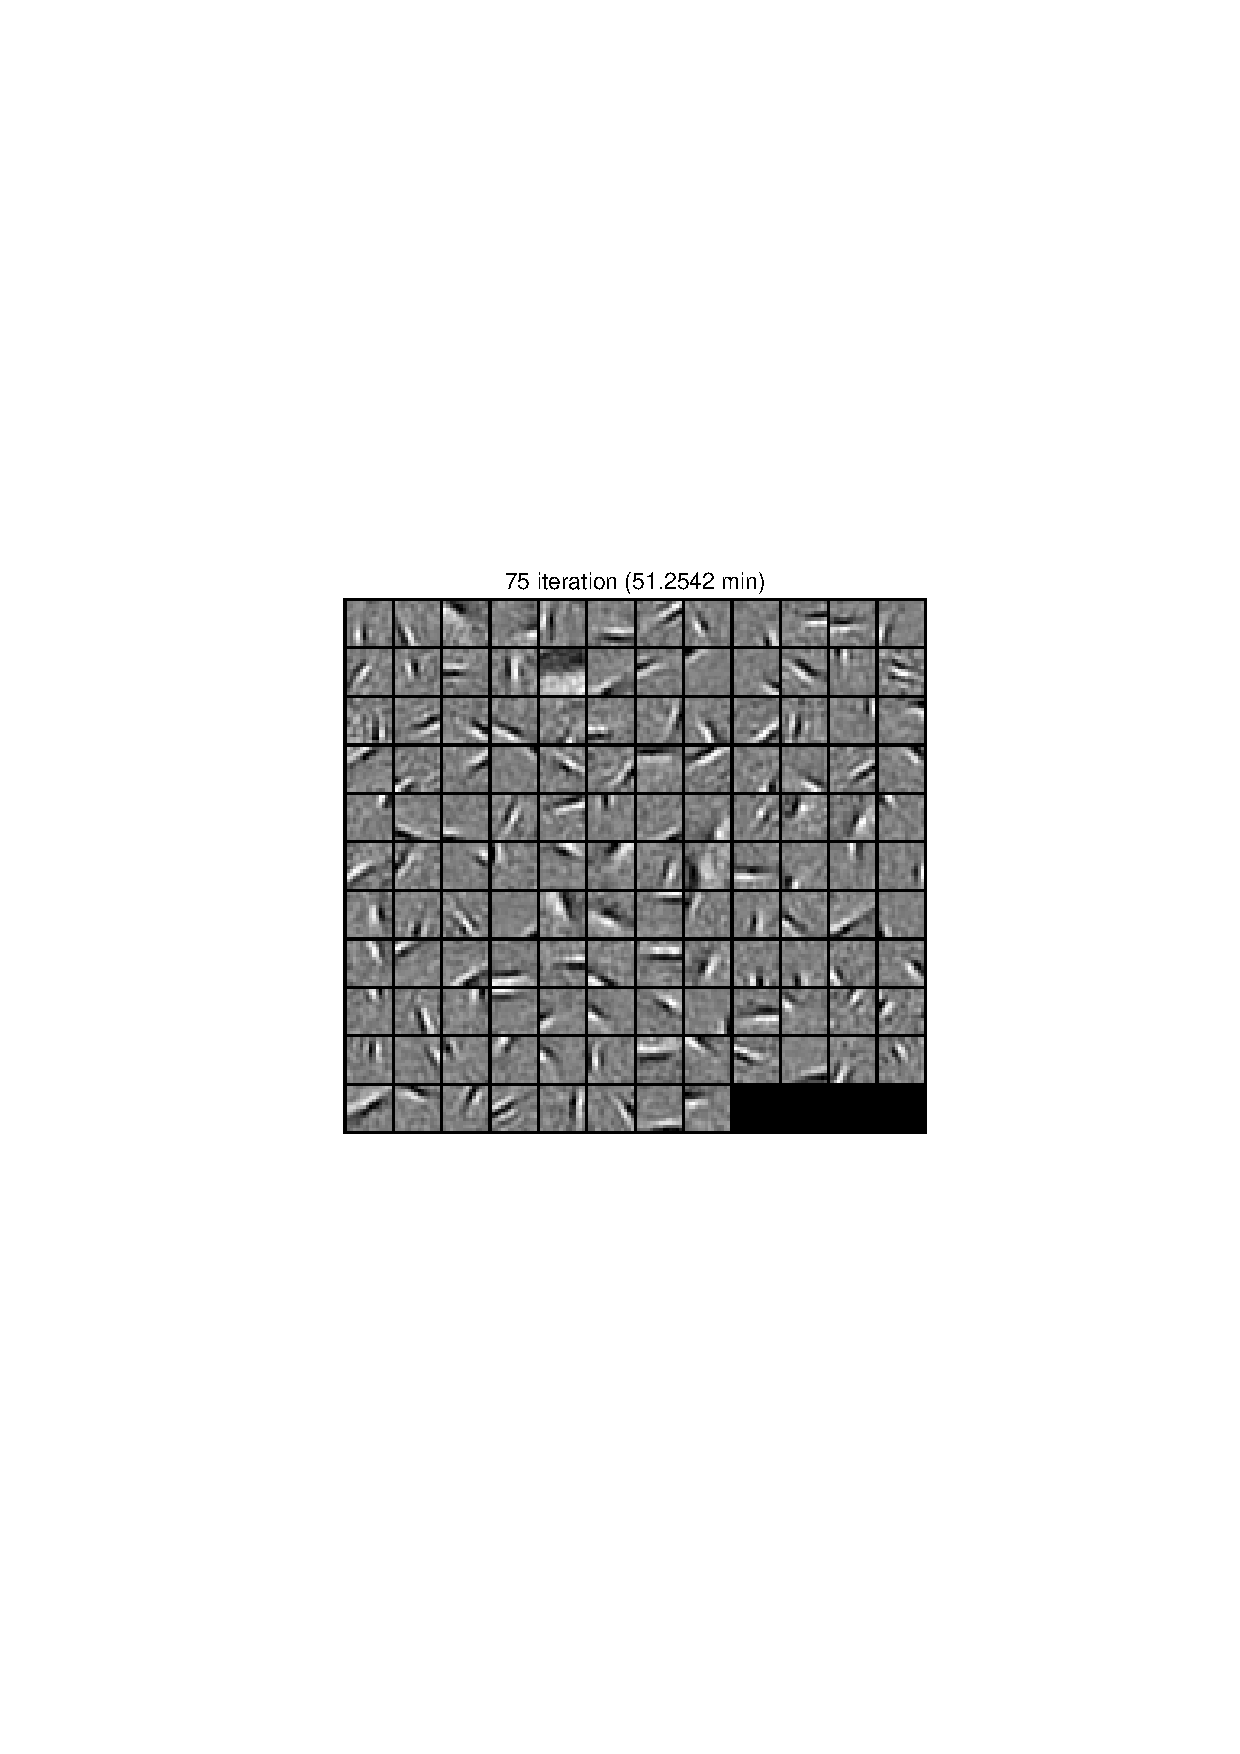
\includegraphics[width=8cm]{fig/128_12.pdf}
%\caption{算法学到的边缘特征}
\label{fig1}
\end{figure}
该图了展示了算法学到的128个基(每个基都是由$14\times14$个像素点组成),迭代了75次,花费51分钟。

通过这128个基的线性组合,基本上可以将原图片给还原出来,可以看出算法学到的基都是一些边缘图像,这与人类大脑类似,神经生理研究表明:在
初级视觉皮层(Primary Visual Cortex)下细胞的感受野具有显著的方向敏感性,单个神经元仅对处于其感受野中的刺激做出反应,即单个神经元仅对某一频段的信息呈现较强的反映,如特定方向的边缘、 线
段、 条纹等图像特征。

此外,尽管我们选取作为训练集的照片不同,但最后提取出来的特征都是类似的,也说明了这种边缘特征的存在是具有普遍性的,在稀疏性的限制下更有利于其他图像结构的表达。

\begin{figure}[H]
\centering
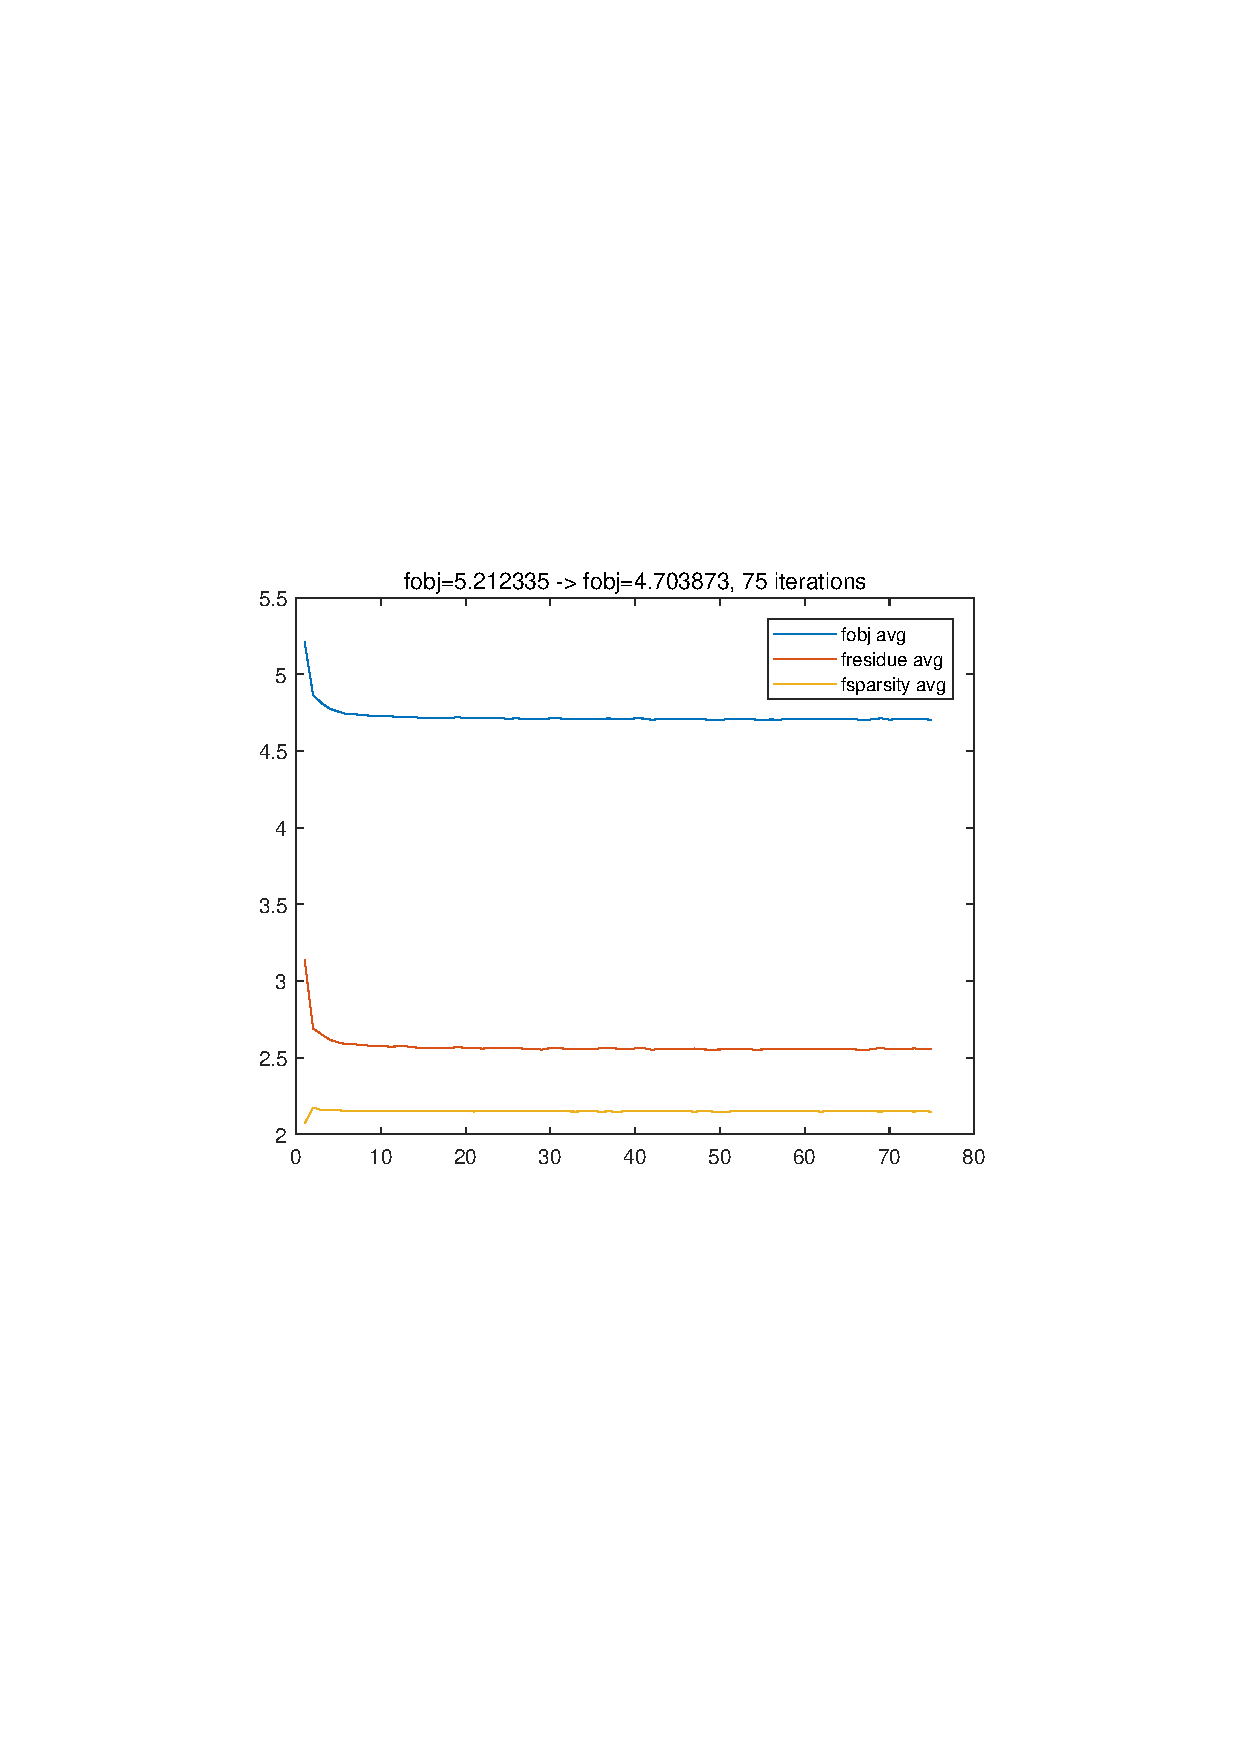
\includegraphics[width=8cm]{fig/128_22.pdf}
\caption{目标函数、重构误差、稀疏惩罚值的下降情况}
\end{figure}

\begin{figure}[H]
\centering
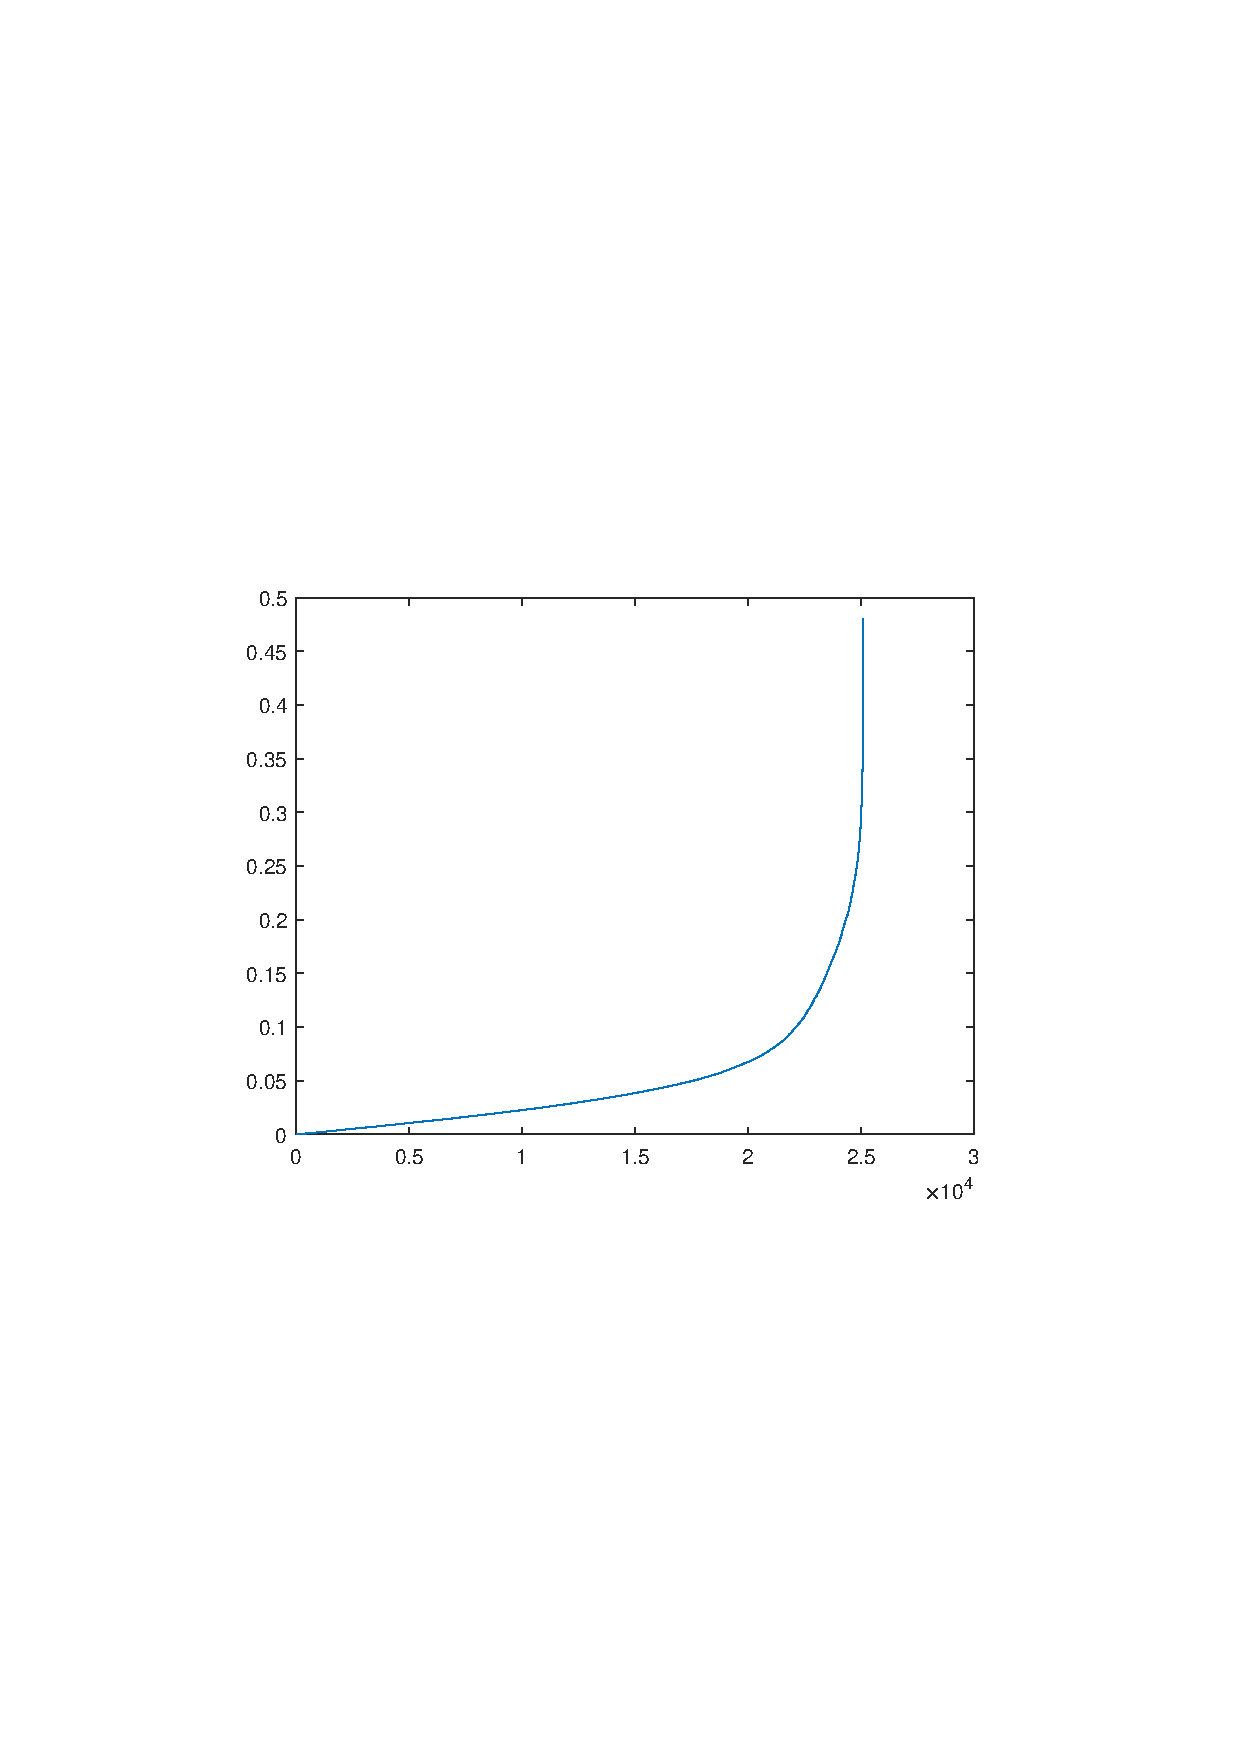
\includegraphics[width=8cm]{fig/128_32.pdf}
\caption{$S_{i,j}$排序后输出的值}
\label{fig3}
\end{figure}

\begin{figure}[H]
\centering
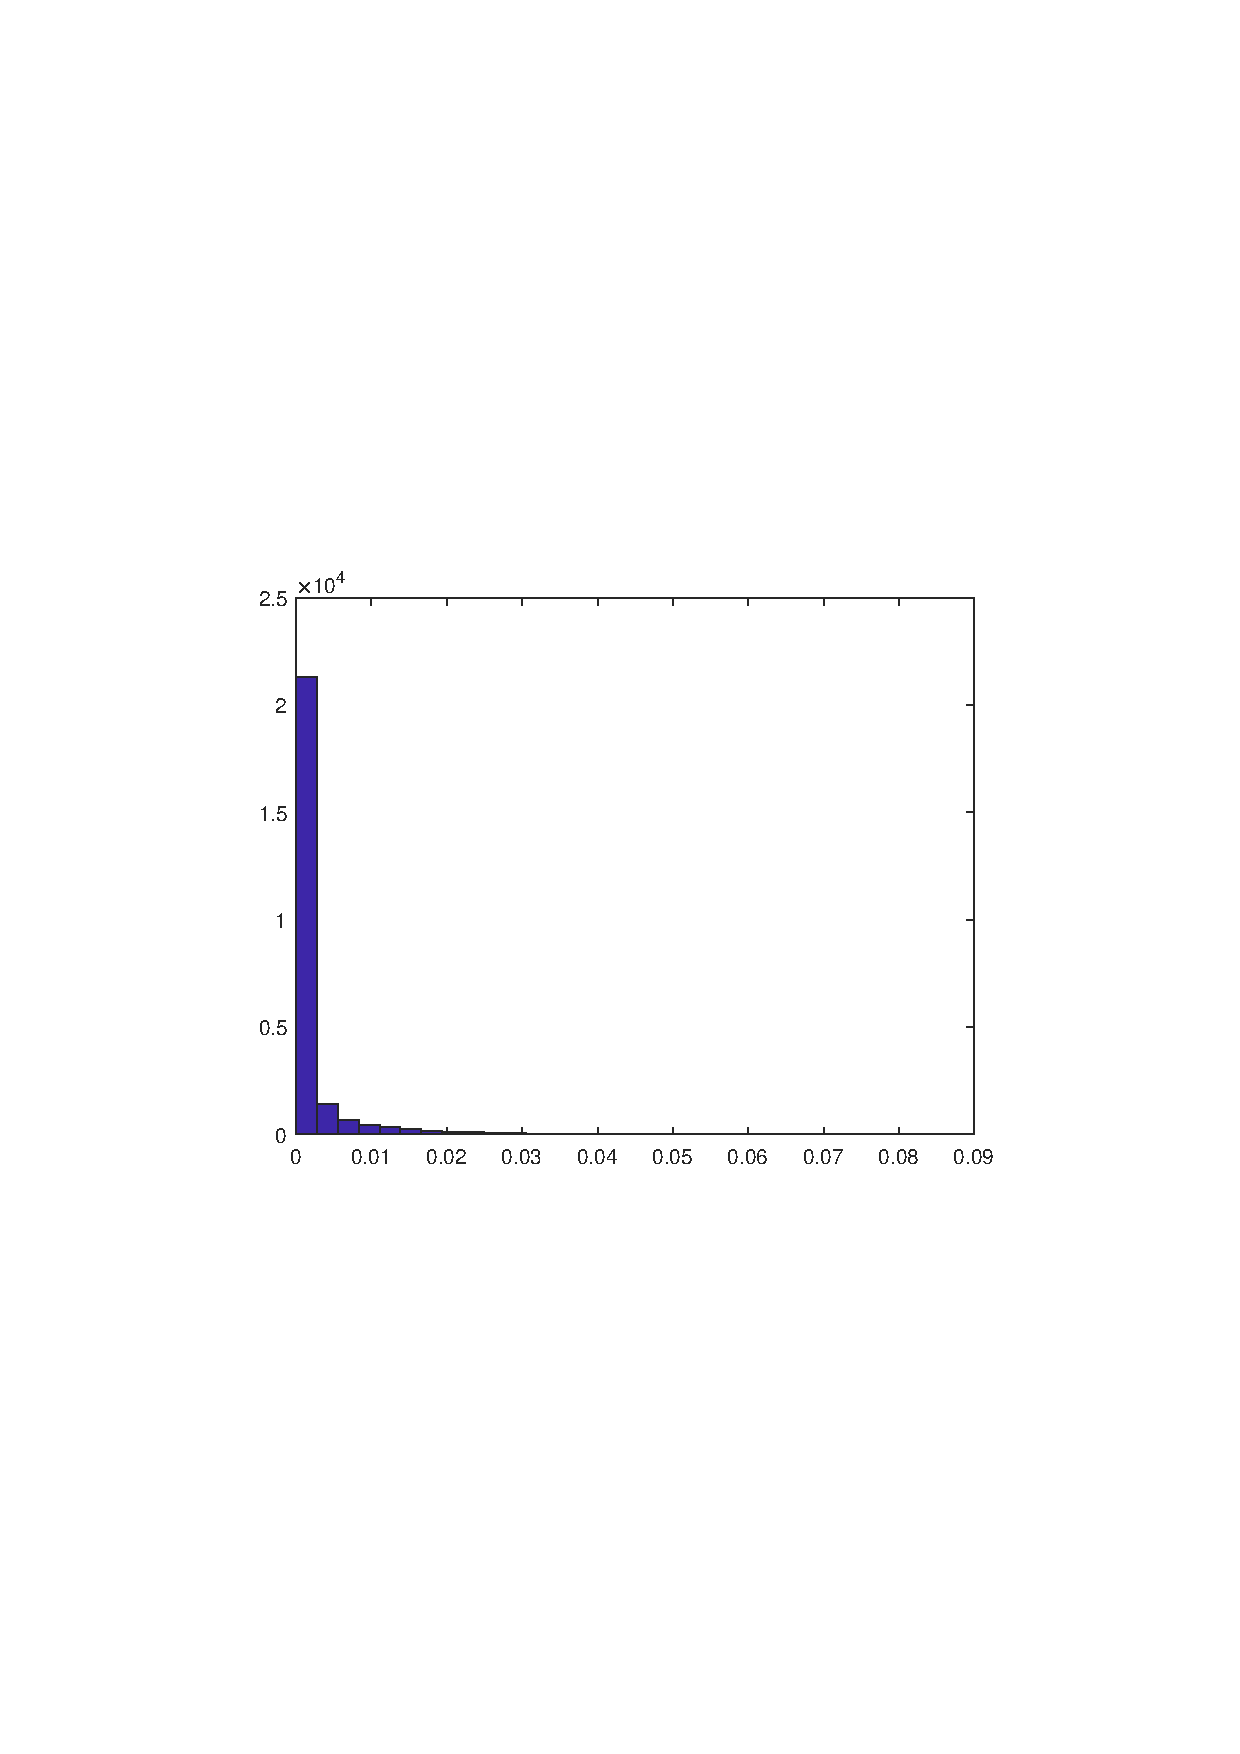
\includegraphics[width=8cm]{fig/128_42.pdf}
\caption{$S_{i,j}$的HuberLoss损失函数直方图}
\label{fig4}
\end{figure}

从图\ref{fig3}可以看出来,系数$S$的分布有$4/5$都在0.06以下,图\ref{fig4}更是说明大部分系数都是集中在0附近,满足了稀疏性的要求。

\appendix
%\appendixpage
\addcontentsline{toc}{chapter}{附录}
\section{HuberLoss函数}
HuberLoss是一个用于回归问题的带参数的损失函数。

\begin{equation*}
  L_{\delta}(y,f(x))=\left\{
    \begin{array}{ll}
    \frac{1}{2}(y-f(x))^2 & \text{if}\, |y-f(x)|\leq \delta, \\
      \delta|y-f(x)| -\frac{1}{2}\delta^2 & \text{if}\, |y-f(x)|> \delta.
    \end{array}
  \right.
\end{equation*}

$\delta$是 HuberLoss 的参数,$y$ 是真实值,$f(x)$ 是模型的预测值。
当预测偏差小于 $\delta $时,它采用平方误差,当预测偏差大于$\delta$的时候,采用的线性误差。相比于最小二乘的线性回归,HuberLoss 降低了对 outlier 的惩罚程度,所以 HuberLoss 是一种常用的 robust regression 的损失函数。
\begin{minted}[breaklines,frame=lines,linenos]{matlab}
%绘制HuberLoss函数的代码
diff = linspace(-4, 4, 1000);
hold on
plot(diff,0.5.*diff.^2)
plot(diff, (abs(diff)<1).*0.5.*diff.^2+(abs(diff)>1).*(abs(diff)-0.5))
legend('0.5x^2','Huber loss')
\end{minted}
\begin{figure}[H]
\centering
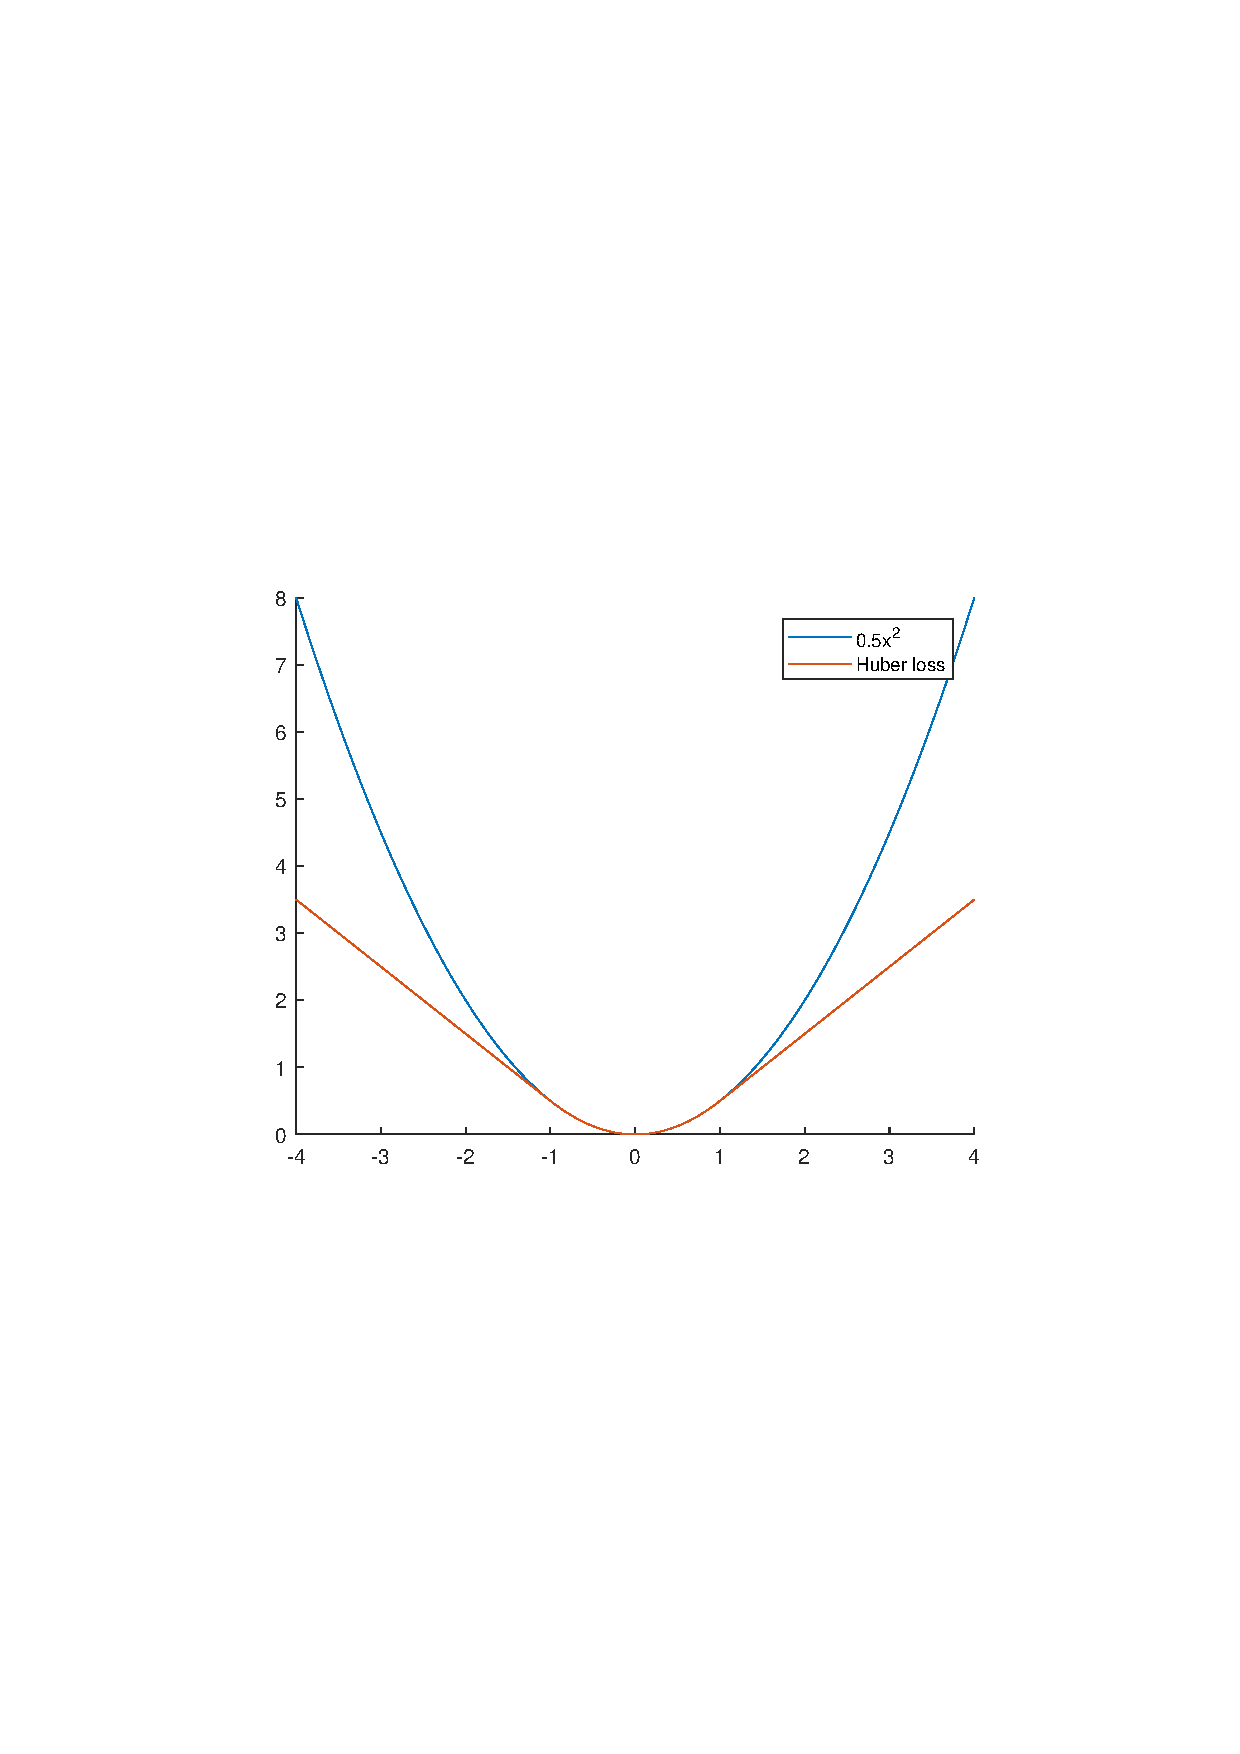
\includegraphics[width=9cm]{fig/HuberLoss.pdf}
\caption{HuberLoss损失函数}
\end{figure}

\section{Andrew Ng对于稀疏编码的说明}
V1区是大脑视觉处理的第一阶段,
V1中的神经元经起到的\textbf{边缘检测器作用(edge detectors)},当瞳孔发现了眼前的物体的边缘,而且这个边缘指向某个方向时,对应的V1神经元细胞就会开始活跃。

同时,更复杂的结构也能很好地被这些边缘特征线性表达,而将复杂结构组合起来就能表达更复杂的结构,也就是说高层的特征是低层特征的组合。

例如,当人眼看到一个气球时,视网膜得到了最基本的信息——像素点(由瞳孔摄入),接着像素点组合成了边缘和方向(被V1区细胞感知),然后大脑判定眼前的物体的形状是圆形的(由V2区细胞感知形状),最后进一步判定该物体是只气球(由V3、V4等区域感知更高级更抽象的特征)。

\begin{figure}[H]
\centering
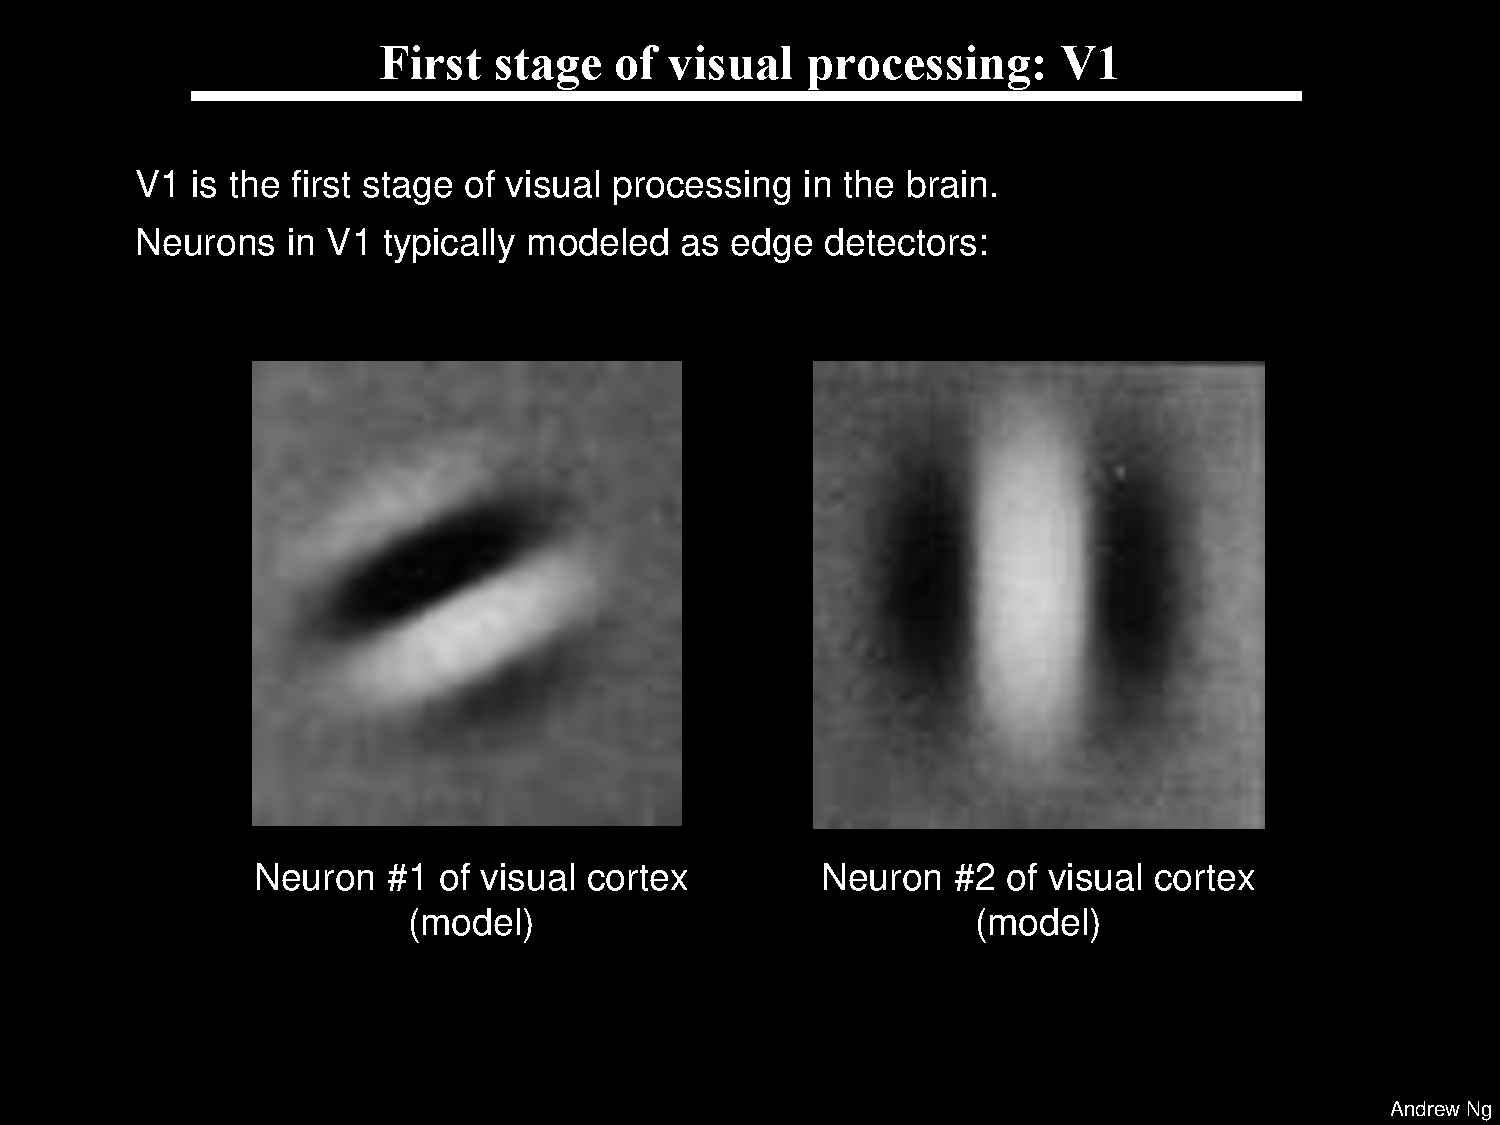
\includegraphics[width=12cm]{fig/ref1.pdf}
\end{figure}
\begin{figure}[H]
\centering
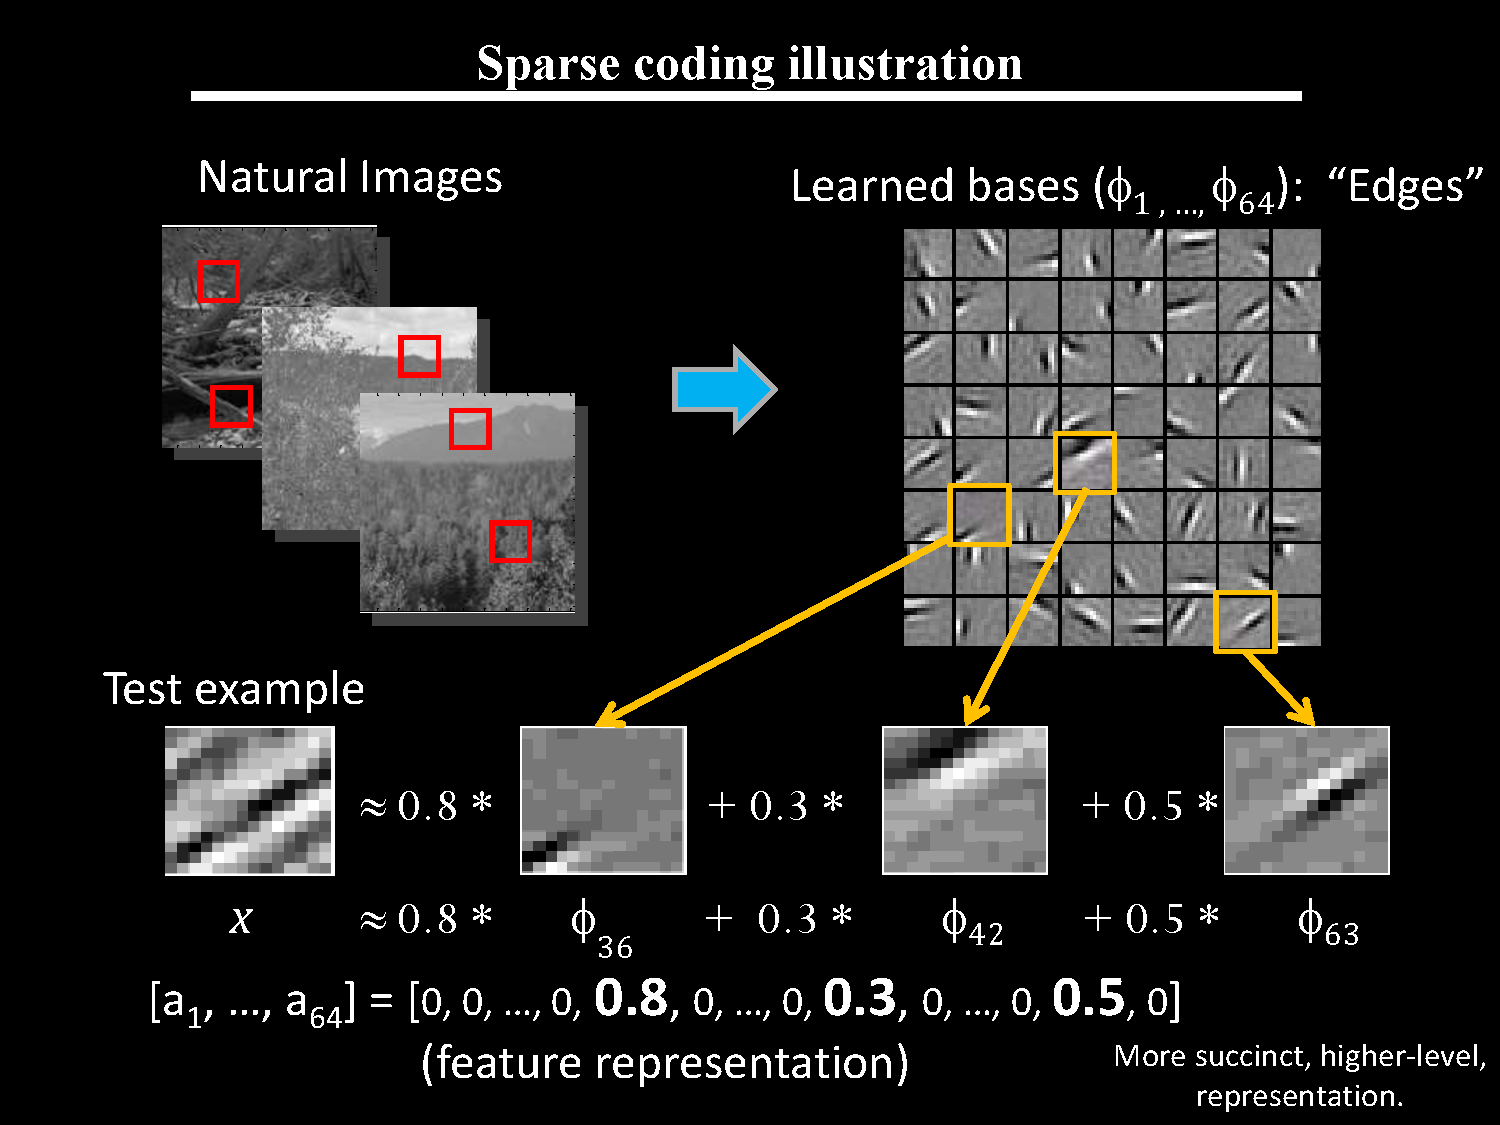
\includegraphics[width=12cm]{fig/ref2.pdf}
\end{figure}
\begin{figure}[H]
\centering
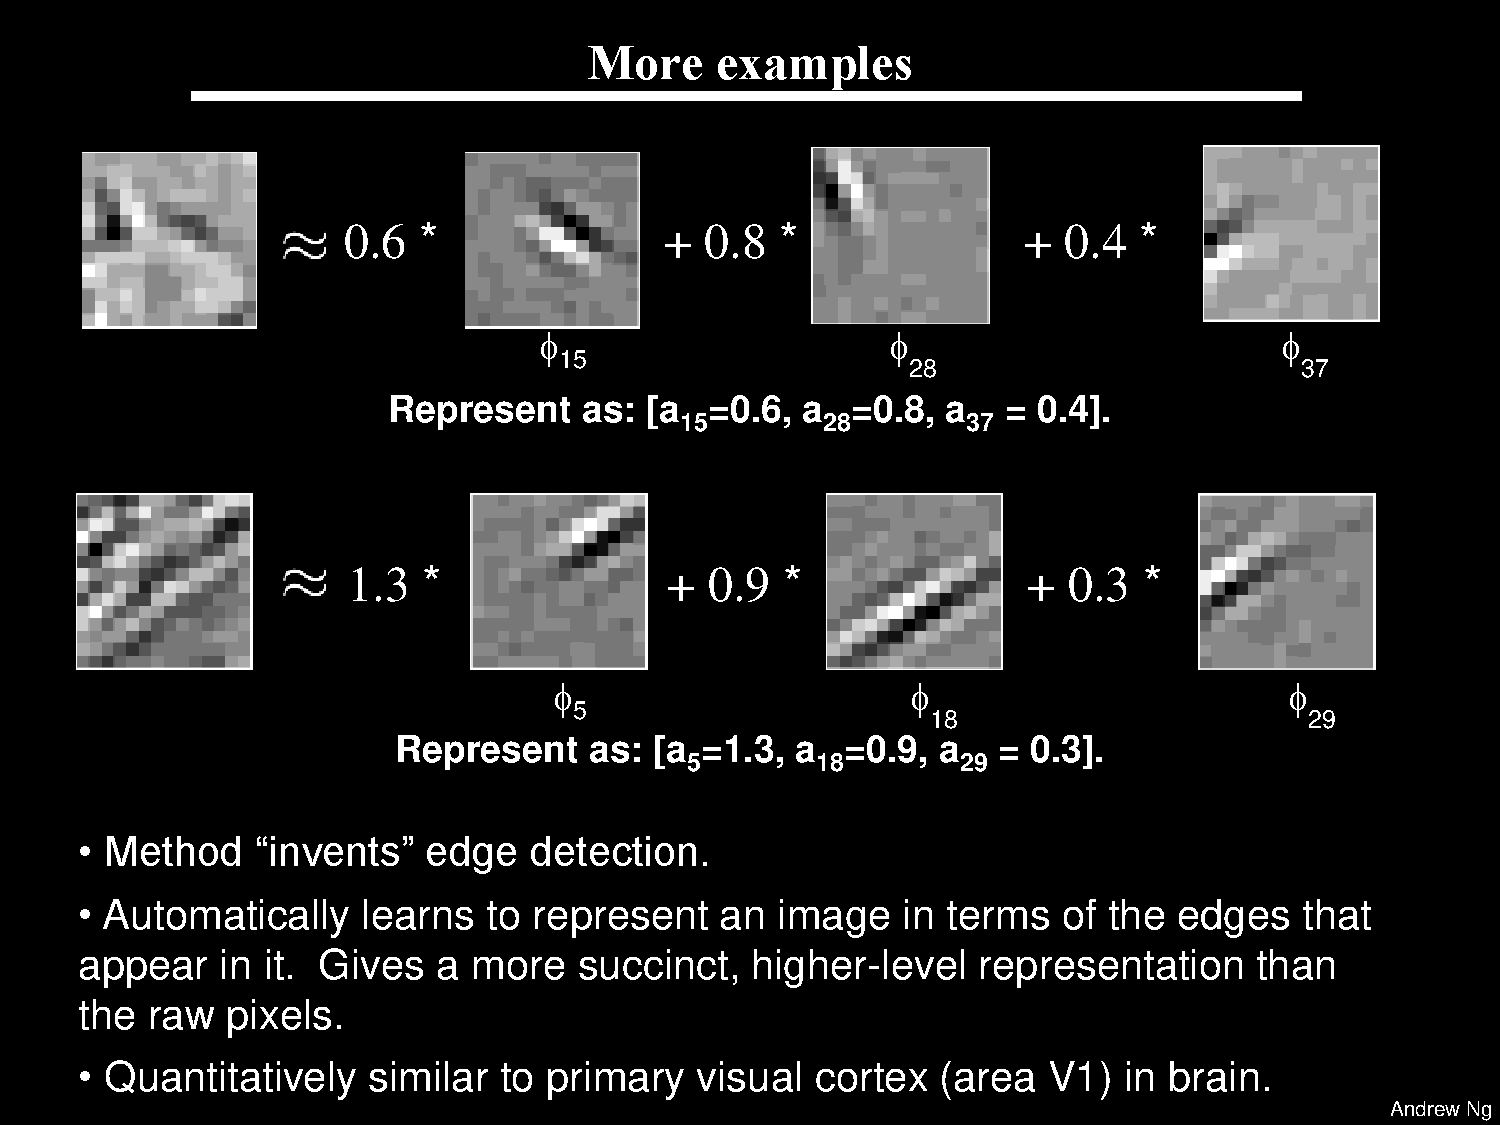
\includegraphics[width=12cm]{fig/ref3.pdf}
\end{figure}

\end{document} 